\chapter{Modeling of Train Operations}
\label{chap:ModelingOfTrainOperations}
\par\noindent
\textit{\textbf{Introduction}} Chapter \ref{chap:FundamentalsOfRailwayVehicleEngineering} has established the theoretical model of the train braking process. It will serve as a foundation to build a practical model suitable for conducting actual simulations. 

\section{Matlab Simulink}
\label{sec:MatlabSimulink}
The model has been built utilizing the software Matlab Simulink by Mathworks. It offers several distinct advantages: It uses a graphical block diagramming tool which makes it very intuitive to use. At the same time, various official and third-party add-on libraries make it very versatile. Most importantly, as it is tightly integrated with the Matlab environment, it can be used for both modeling and simulating dynamical systems, like the braking process of a train.

\section{Initial Model}
\label{sec:InitialModel}
\par\noindent
Looking back at chapter \ref{chap:FundamentalsOfRailwayVehicleEngineering}, the aim is to build a model for the braking process of a freight train. An initial model of a single braking procedure, kindly provided by Dr. Raphael Pfaff, will serve as a basis. Most of the components previously designed in chapter \ref{chap:FundamentalsOfRailwayVehicleEngineering} can already be found therein.  

\begin{figure}[H]
	\centering
	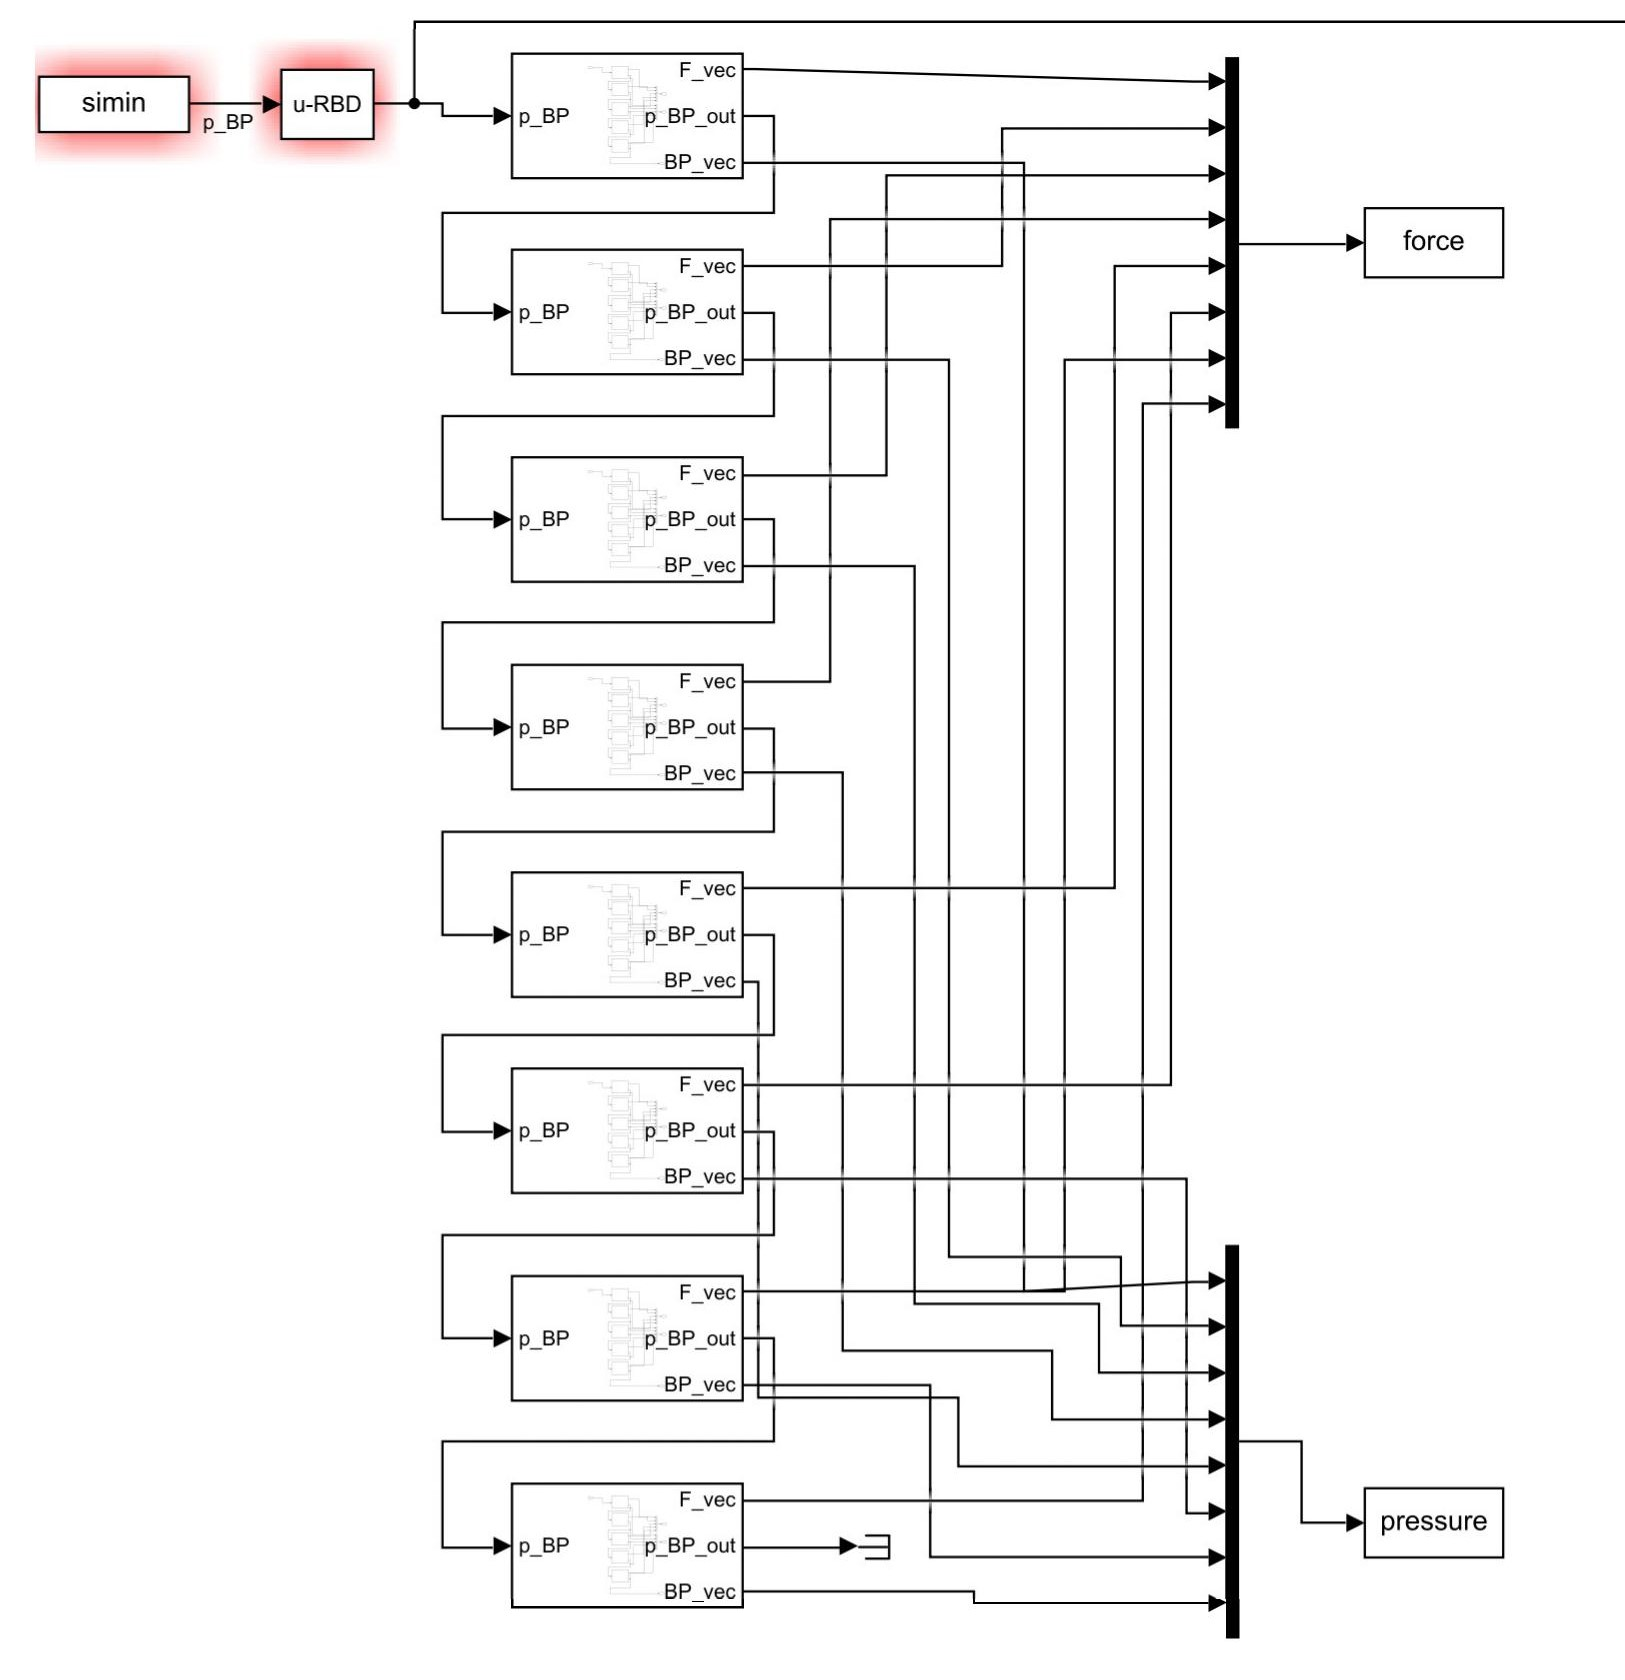
\includegraphics[width=\linewidth]{./pic/initmodel_whole}
	\caption{Initial Model}
	\label{fig:initmodel_whole}
\end{figure}

\par\noindent
Figure \ref{fig:initmodel_whole} shows a model of a freight train of fixed length, consisting of 40 wagons in total. For better readability, five wagons are condensed into one subsystem each, marked by the red rectangle. The subsystems are interconnected by a brake pipe, marked by the green arrow. They have one input port for the incoming pressure on the brake pipe, and three output ports, one for the pipe connection to the next subsystem, and two for recording brake pressure and brake force (marked by the pink and blue arrows, respectively). A depiction of a subsystem can be found in appendix \ref{fig:initmodel_subsys}.  

\begin{figure}[H]
	\centering
	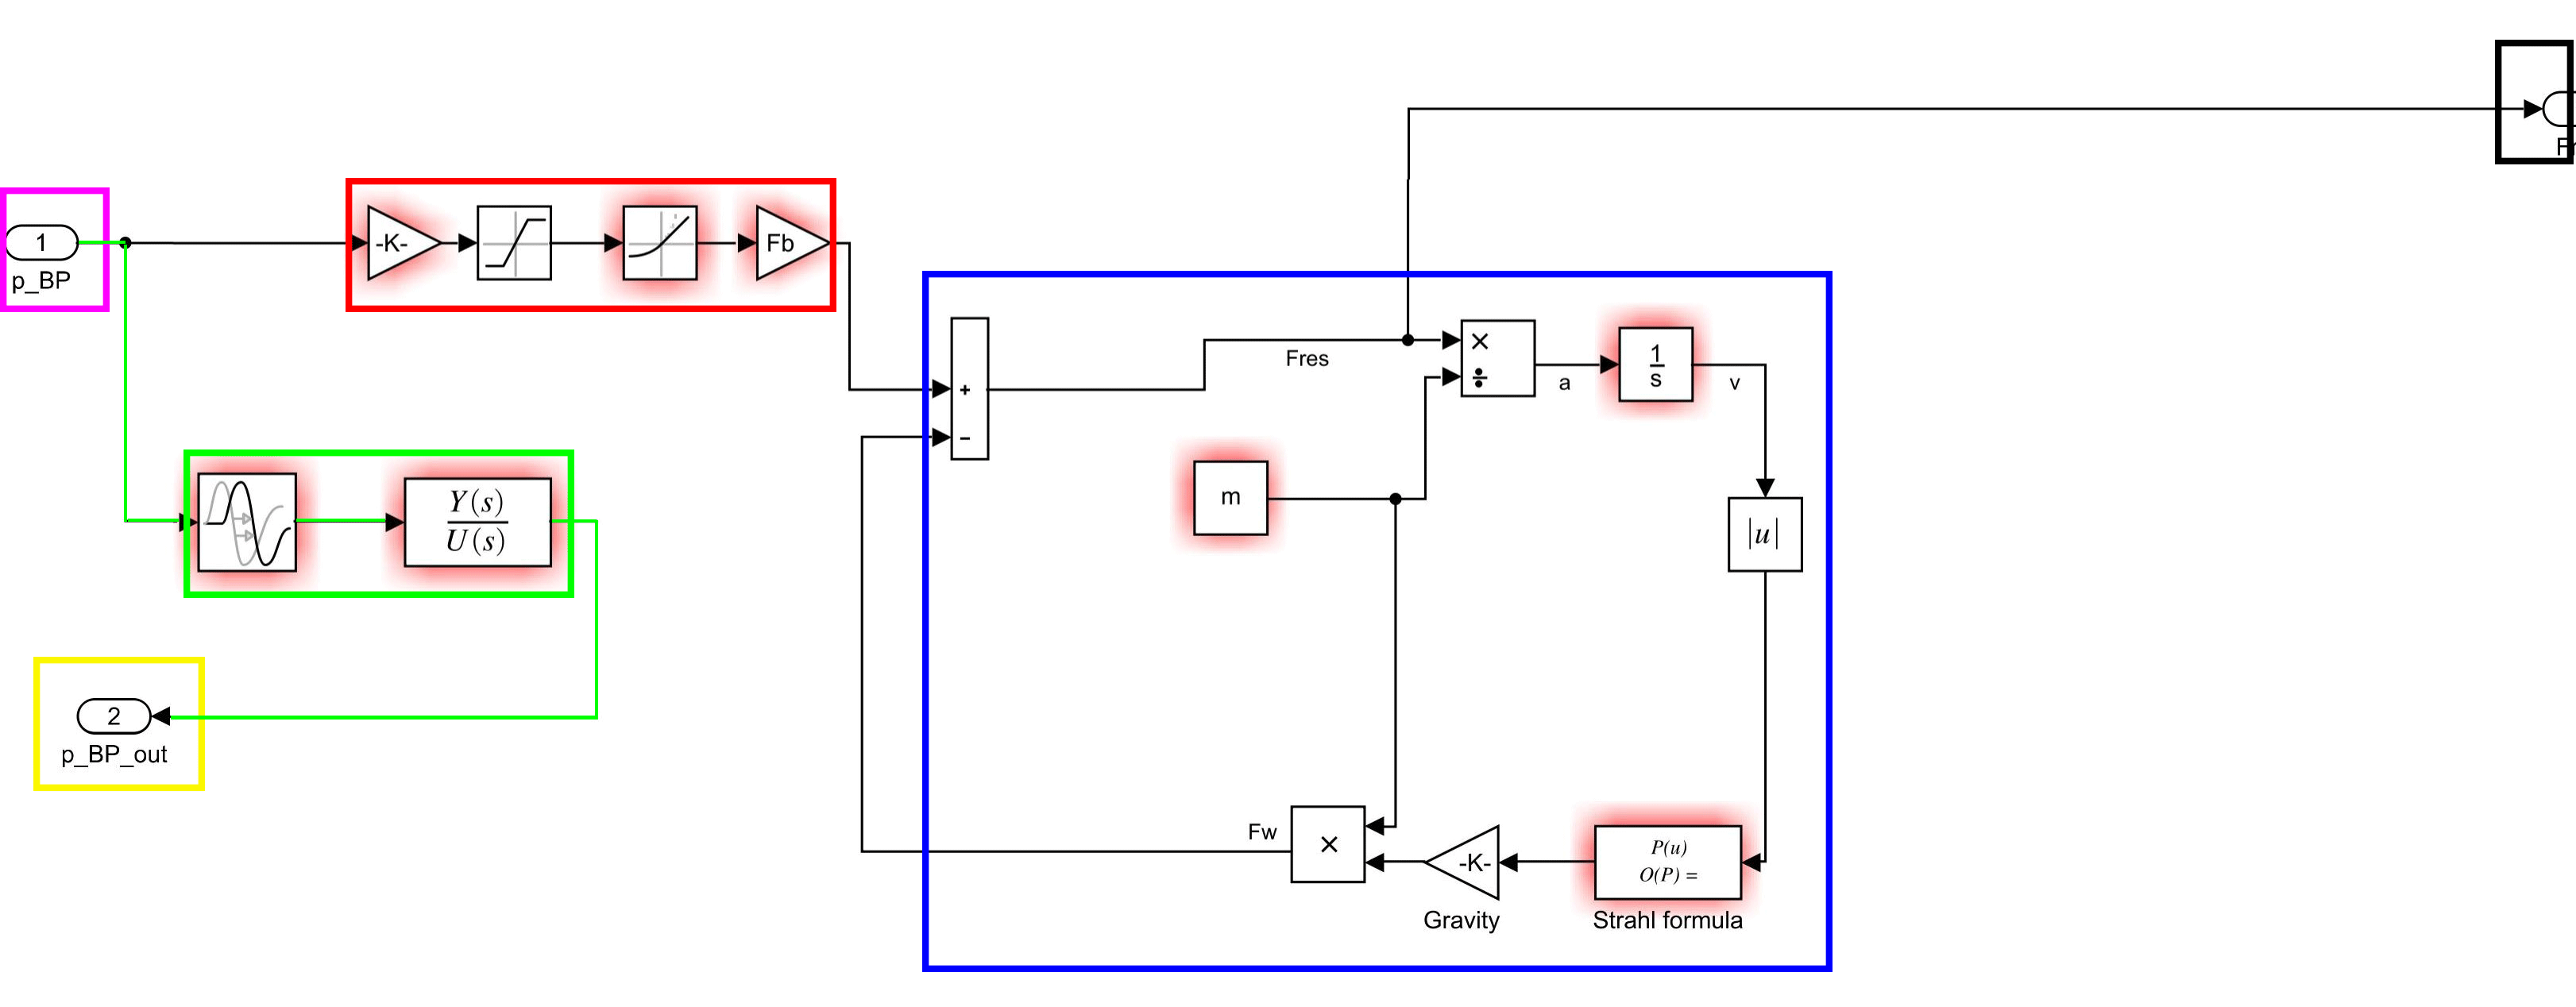
\includegraphics[width=\linewidth]{./pic/initmodel_wagon}
	\caption{Initial Model - Wagon}
	\label{fig:initmodel_wagon}
\end{figure}

\par\noindent
Figure \ref{fig:expandedmodel_wagon} shows a model of a freight wagon. It already encompasses several of the model variables defined in section \ref{sec:InherentFactors}. The brake pipe ${\mathcal{M}}_{bp}$ is represented by the green arrows. It leads from input port (pink rectangle) to output port (yellow rectangle); the propagation delay is realized by a transport delay block (green rectangle), using propagation velocity $v_{bp}$ and wagon length $l_{bp}$. The brake pressure $p_{bp}$ is the value of the signal traveling through the connection. Note that in the simulation, the signal value for $p_{bp}$ is the difference between regular operating pressure and actual pressure, e.g. if simulated pressure on the brake pipe is 3.5 bar, the signal value is $3.5 - 5 = -1.5$.
\par
The brake cylinder ${\mathcal{M}}_{bc}$ is represented by the red rectangle. The pressure on the brake pipe $p_{bp}$ is converted into a coefficient between zero and one, where zero equals no brakes applied, or $p_{bp} = 5$, and one equals full braking pressure, or $p_{bp} = 3.5$. The exact formula is this:

\begin{align*}
p_{bc} = p_{bp} \cdot \frac{-1}{5-3.5}
\end{align*}

\noindent
So for a braking pressure of 4 bar, the coefficient would be $(4 - 5) \cdot \frac{-1}{5-3.5} = -1 \cdot \frac{-1}{1.5} = \frac{2}{3}$. A rate limiter block accounts for the brake cylinder's filling time $t_{bc}$. Finally, the braking force is calculated by multiplying the maximum braking force, which is mainly dependent on the wagon mass $m$ [train braking, 22]. So for the braking pressure, we have:

\begin{align*}
F_{b} = F_{b,max} \cdot p_{bc}
\end{align*}

\noindent
The final component is the factoring in of the driving resistance of the train, utilizing Strahl's formula. This is represented by the blue rectangle. By continuous-time integration of the acceleration, which is calculated according to Newton's second law of motion ($a = \frac{F}{m})$, it is possible to determine the velocity, which in turn allows for the calculation of the force generated by the driving resistance, This force is then added to the braking force and fed into an output port, marked with the black rectangle.
\par
Regarding simulation, this initial model is only fit for one single braking process, where a train of fixed length and fixed composition, brakes from an initial velocity all the way to a halt; the only variation is the pressure on the brake pipe, which is also the sole input for the simulation. Appendix \ref{fig:initmodel_input} shows how that input might look like.

\section{Model Expansion}
\label{sec:ModelExpansion}

\par\noindent
This initial model is however not of sufficient detail. Where it merely simulates a single, rather undynamic braking process, the goal is the simulation of a train ride, with alternating phases of braking and accelerating. The model should furthermore factor in more components of the theoretical model ${\mathcal{M}}$ discussed in chapter \ref{chap:FundamentalsOfRailwayVehicleEngineering}, as well as allow for the recording of more properties specific to the braking process. For that purpose, the model has to be expanded. The simulation input needs to be changed in order to allow for the simulation of a train ride. Previously, it being only one braking process, using braking pressure as input was the obvious choice. This will be replaced by a track profile, according to which the train either engages its brakes, or accelerates. This will be discussed in further detail in chapter \ref{chap:DataGeneration}.
\par
In the initial model, the train is only able to decelerate by engaging its brakes. To allow for acceleration, it is necessary to expand the model accordingly. This may be realized by a rather simple two-point controller, which means the train is either accelerating or decelerating. The decision on whether to engage brakes or apply traction force at a particular point in time is made utilizing the track profile: If the current velocity of the train $v_{real}$ is greater than the maximum allowed velocity $v_{max}$ at that time, the train engages its brakes by lowering the pressure on the brake pipe $p_{bp}$. If $v_{real}$ is less than $v_{max}$, the train applies a traction force $F_{t}$ in order to increase speed. Both $p_{bp}$ and $F_{t}$ scale with the discrepancy between $v_{real}$ and $v_{max}$. This means the higher the value of $v_{dif}$ is, the more pressure is vented from the brake pipe (or the more traction force is applied). This prevents the train from overcompensating, for example applying full braking pressure to decrease velocity by $2 \; \frac{m}{s}$. Notice there is actually no case for when $v_{real}$ equals $v_{max}$, i.e. $v_{dif} = 0$. One might expect that this would lead to the train constantly oscillating between accelerating and decelerating, but in practice this does not occur, and it is thus unnecessary to account for that case.

\begin{figure}[H]
	\centering
	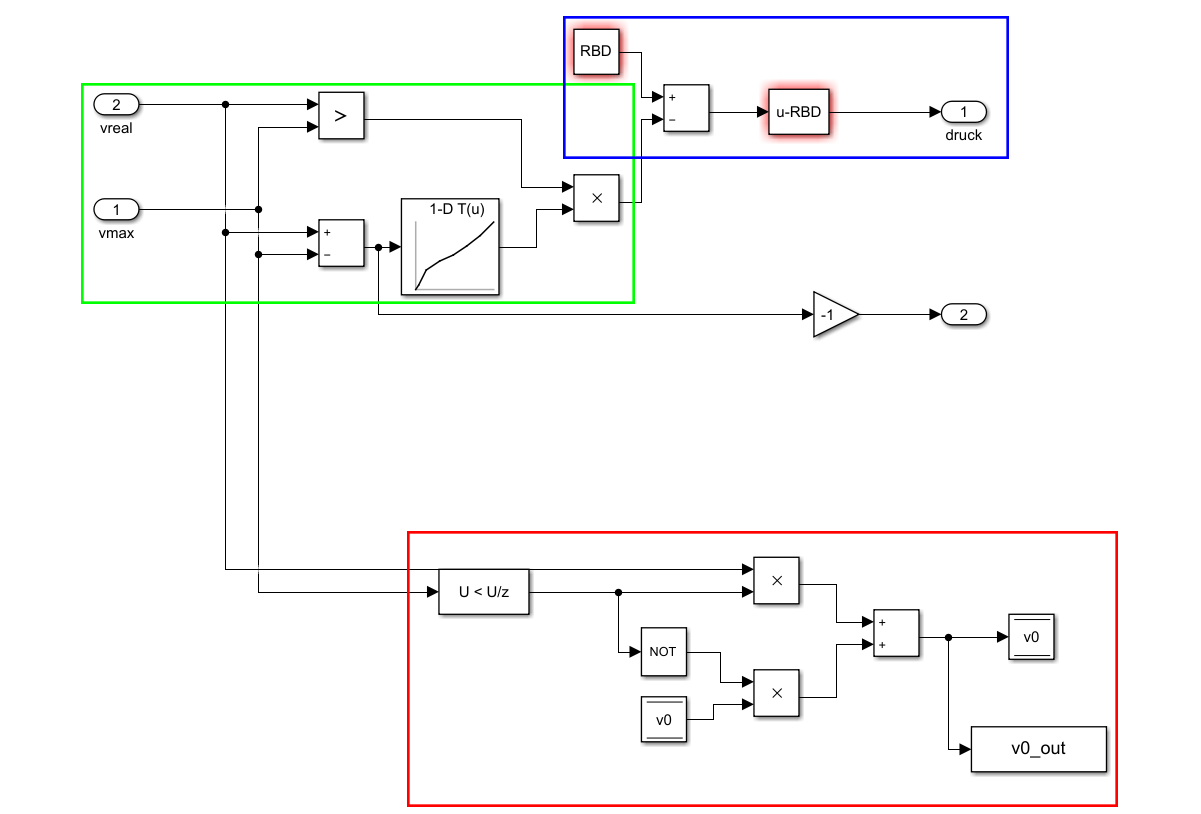
\includegraphics[width=\linewidth]{./pic/expandedmodel_pressure}
	\caption{Expanded Model - Pressure Calculation}
	\label{fig:expandedmodel_pressure}
\end{figure}

\par\noindent
Figure \ref{fig:expandedmodel_pressure} shows the subsystem responsible for the calculation of the braking pressure $p_{bp}$. The difference between $v_{real}$ and $v_{max}$ is used as input for a one-dimensional lookup table, which in essence is a step-function mapping different input values to discrete output values. 

\begin{equation}
\label{eq:lookuptable}
H(n) =
\begin{cases}
0.1 & \text{if $n=1$} \\
0.7 & \text{if $n=15$} \\
0.8 & \text{if $n=20$} \\
\text{..}
\end{cases}
\end{equation}

\noindent
Equation \ref{eq:lookuptable} is an example for how this function might look like. The input parameter $n$ stands for the discrepancy between actual and maximum velocity $v_{dif}$, and the output of the $H(n)$ represents the amount of pressure to vent from the brake pipe. This allows for adjusted braking, where $p_{bp}$ is directly proportional to $v_{dif}$.
\par
To account for the train only engaging its brakes in case its current velocity is higher than the maximum allowed velocity, a relational operator $>$ is used to compare $v_{real}$ to $v_{max}$.

\begin{equation}
\label{eq:brakingpressure}
P(n,t) = H(n) \cdot (v_{real}(t) > v_{max}(t))
\end{equation}

\noindent
Equation \ref{eq:brakingpressure} describes the logic. The braking pressure for a velocity discrepancy $n$ at a point in time $t$ equals the result of $H(n)$ (equation \ref{eq:lookuptable}) multiplied with the result of the relational operation comparing $v_{real}(t)$ to $v_{max}(t)$, which is 1 if $v_{real}(t)$ is greater than $v_{max}(t)$, and otherwise 0. This ensures that $P(n,t)$ is zero when the train's velocity is lower than the maximum allowed velocity, and thus no pressure is vented from the brake pipe, and no brakes are engaged. This part of the system is marked by the green rectangle in figure \ref{fig:expandedmodel_pressure}. The blue rectangle marks the conversion of the braking pressure into a signal fit for further calculations, analogous to the initial model, discussed previously. Finally, the red rectangle marks the component for storing the initial velocity of a braking process, which is needed to calculate the braking distance further down the line. This is achieved by using a block to detect a decrease of $v_{max}$, i.e. the block outputs a signal of 1 or 0, accordingly. 

\begin{equation}
\label{eq:initialvelocity}
v_{0} = v_{real} \cdot b + v_{0,old} \cdot \bar{b}
\end{equation}

\noindent
Equation \ref{eq:initialvelocity} describes the logic. The initial velocity of a braking process $v_{0}$ equals the train's velocity multiplied with the result of the decrease detection block, denoted as $b$, added with the previously stored initial velocity $v_{0,old}$ multiplied with the inverse of $b$, denoted as $\bar{b}$. If there is a decrease of $v_{max}$, i.e. the train starts braking, we get $v_{0} = v_{real} \cdot 1 + v_{0,old} \cdot 0 = v_{real}$. In any other case, we get $v_{0} = v_{real} \cdot 0 + v_{0,old} \cdot 1 = v_{0,old}$, i.e. the value of $v_{0}$ does not change as no new braking process has begun.
\par
This completes the description of this subsystem. It is worthy to note that, reaching back to chapter \ref{chap:FundamentalsOfRailwayVehicleEngineering}, this is the practical implementation of the brake valve ${\mathcal{M}}_{bv}$.

\begin{figure}[H]
	\centering
	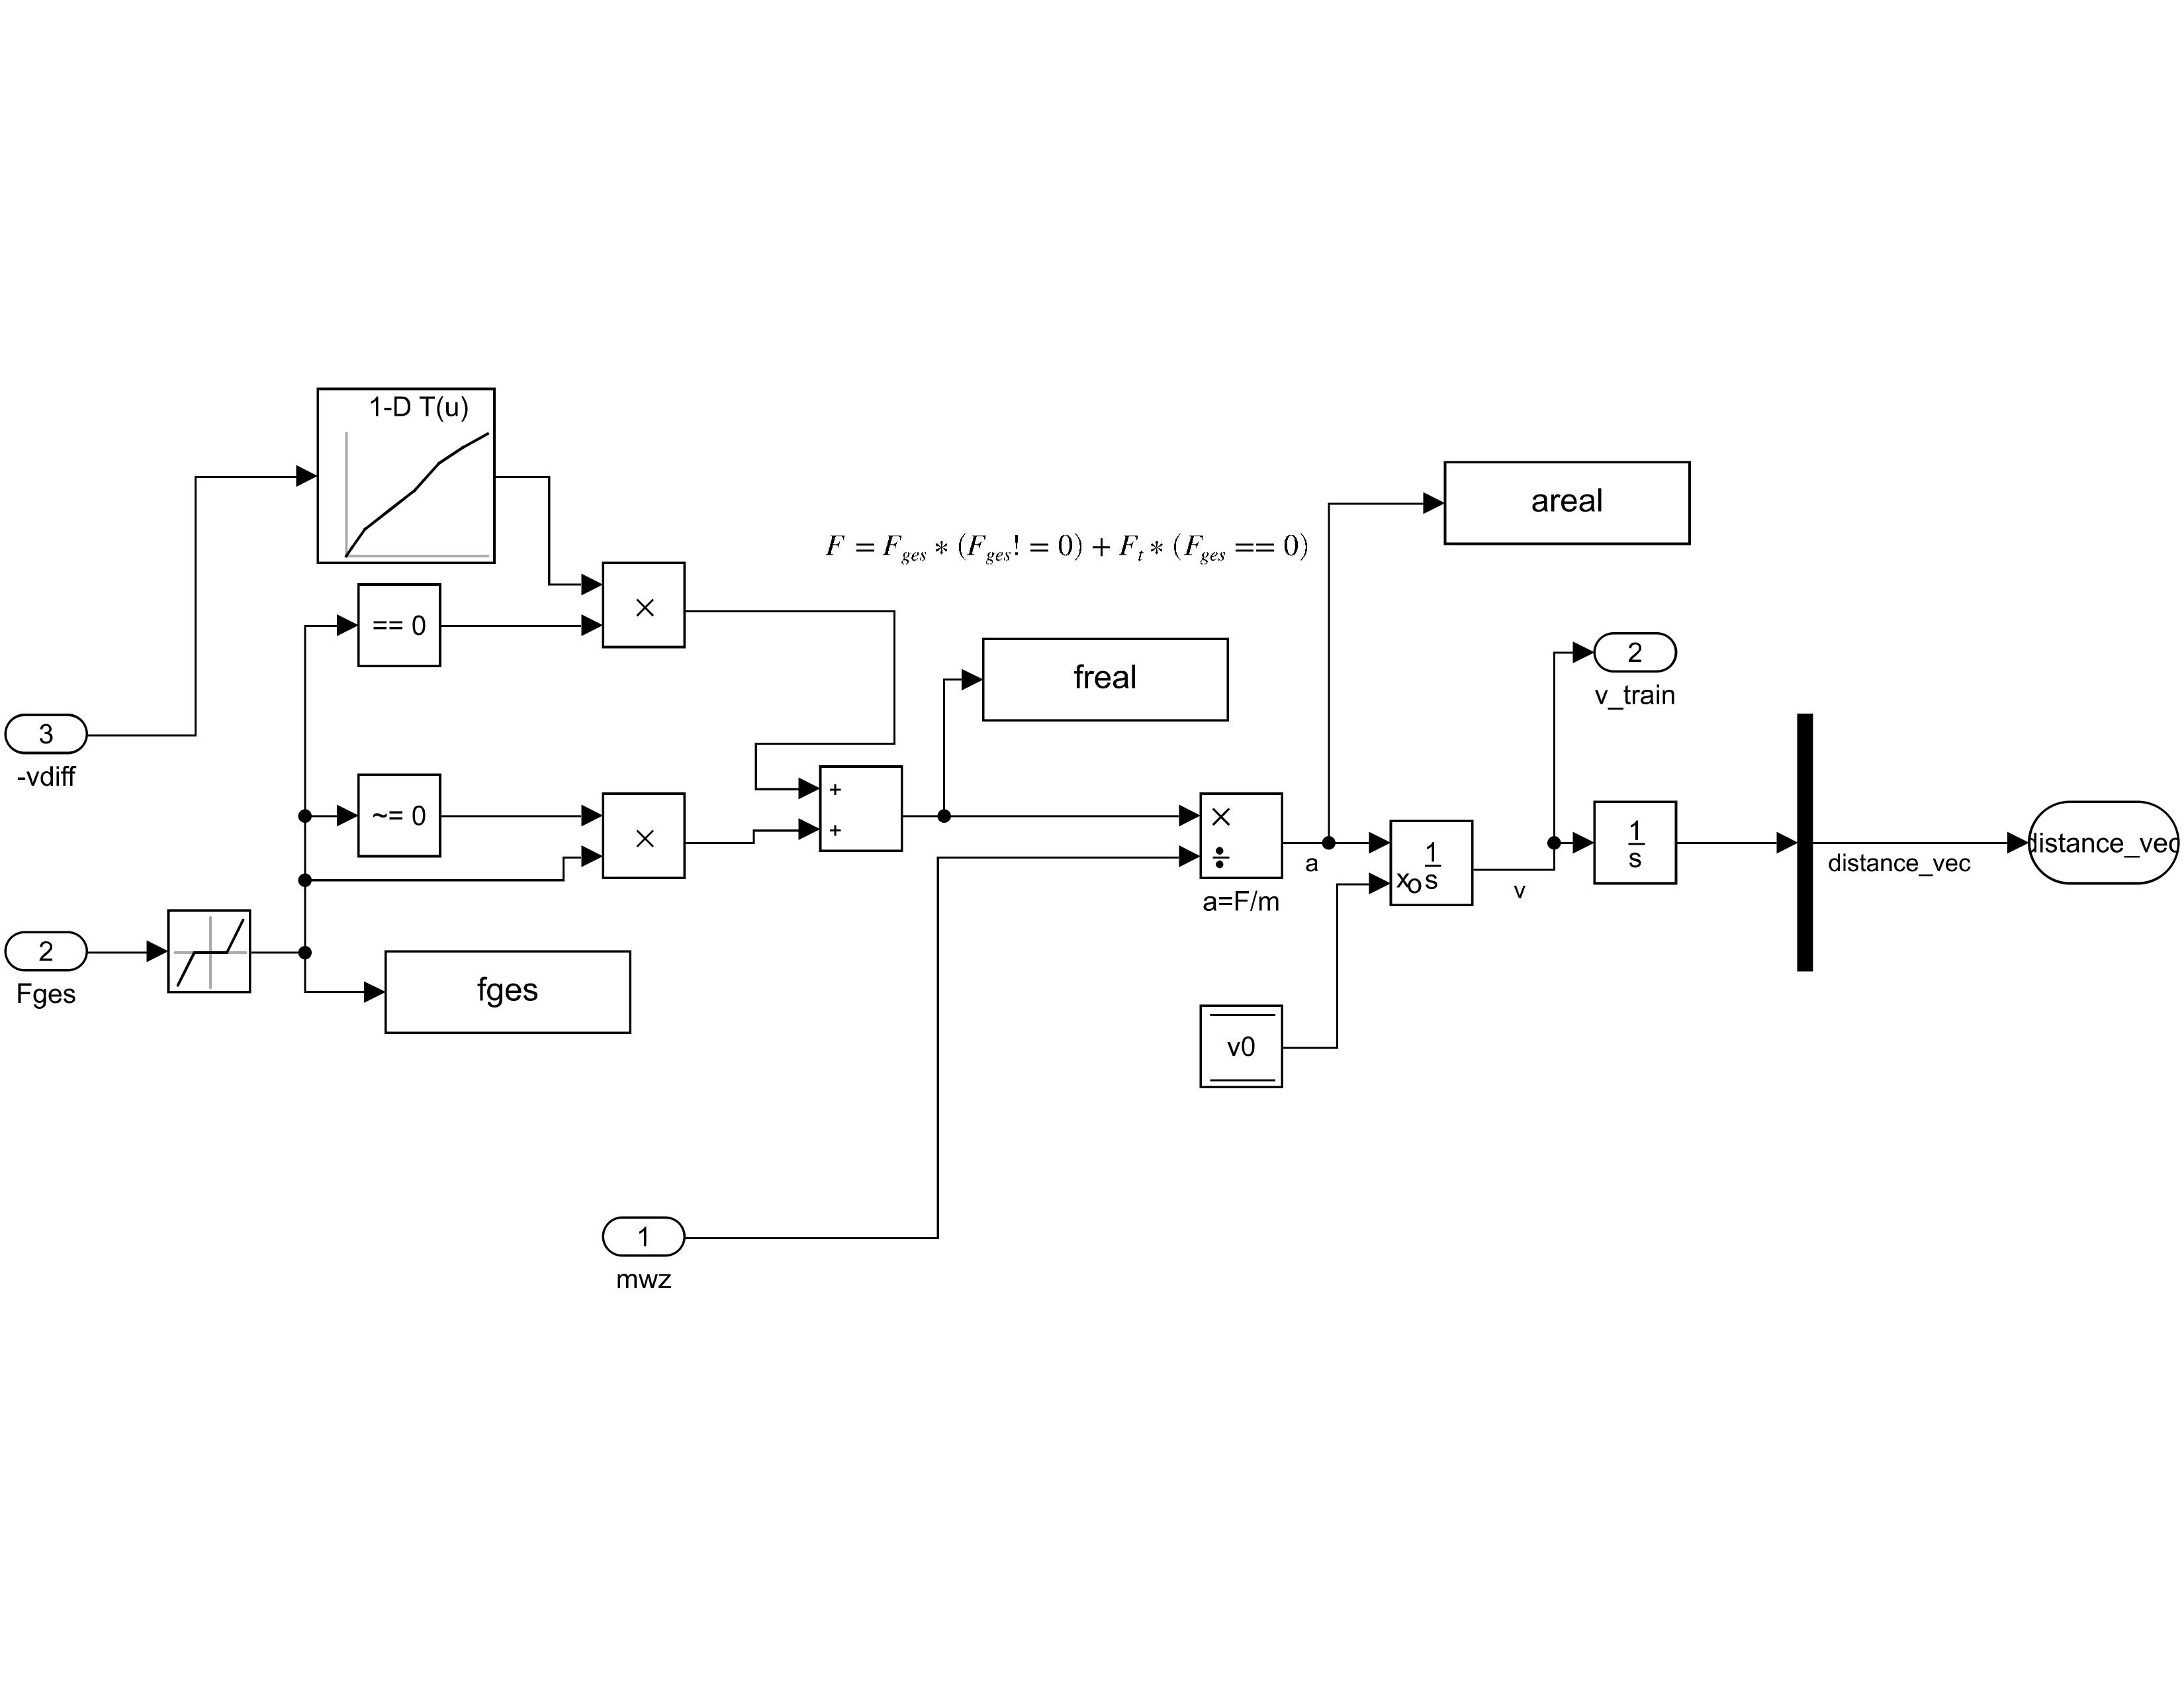
\includegraphics[width=\linewidth]{./pic/expandedmodel_force}
	\caption{Expanded Model - Traction Force Calculation}
	\label{fig:expandedmodel_force}
\end{figure}

\par\noindent
Figure \ref{fig:expandedmodel_force} shows the subsystem responsible for the calculation of the traction force, the train's acceleration, the train's velocity and the train's traveled distance. The applied traction force scales with $v_{dif}$ in a similar fashion to how $p_{bp}$ does. Again, a one-dimensional lookup table is used to calculate the appropriate value for $F_{t}$.

\begin{equation}
\label{eq:lookuptable2}
H(n) =
\begin{cases}
0.05 & \text{if $n=1$} \\
0.45 & \text{if $n=15$} \\
0.6 & \text{if $n=20$} \\
\text{..}
\end{cases}
\end{equation}

\noindent
Equation \ref{eq:lookuptable2} shows an example for how the function for the table might look like. The key difference to the calculation of the braking pressure is that the output values of the function are coefficients which are then multiplied with the maximum possible traction force, rather than raw values like in equation \ref{eq:lookuptable}. This part of the system is marked by the red rectangle.

 As has been discussed earlier, this works like a simple bang-bang controller. The design is very similar to the braking pressure system: $v_{dif}$ is again fed into a one-dimensional lookup table, which outputs different values for traction force accordingly. The higher $v_{dif}$ is, the higher the traction force to apply. It is then added to the current braking force, however only either traction or braking force is at any given time positive while the other is zero, which is achieved by the equations
 
\begin{equation}
\label{eq:tracforce}
f(n,t) = H(n) * (F_{B}(t) == 0) 
\end{equation}

\noindent
where $n$ is $v_{dif}$, $H(n)$ is the lookup table function (see equation \ref{eq:lookuptable}), $F_{B}(t)$ is the braking force over time, and 

\begin{equation}
\label{eq:brakeforce}
g(t) = F_{B}(t) * (F_{B}(t) \neq 0)
\end{equation}

\noindent
where $F_{B}(t)$ is the braking force over time, so we have 

\begin{equation}
\label{eq:force}
F(n,t) = f(n,t) + g(t) 
\end{equation} 

\noindent
where $F$ is the actual force over time, either braking or traction.

\par\noindent
$F$ is then used to calculate acceleration. According to Newton's Second Law,
\begin{equation}
\label{eq:newton}
F = m * a
\end{equation}
Accordingly, acceleration is
\begin{equation}
\label{eq:acceleration}
a = F(n,t) / m
\end{equation}
	
\noindent
where $m$ is the accumulated mass of all wagons and $F(n,t)$ relates to equation \ref{eq:force}. The acceleration is then used to calculate the velocity by integrating $a$ in relation to $v_{0}$, which is the initial velocity of the current braking or acceleration process \TODO{überprüfen..}. Integration of $v$ in turn allows calculation of the traveled distance.

\begin{figure}[H]
	\centering
	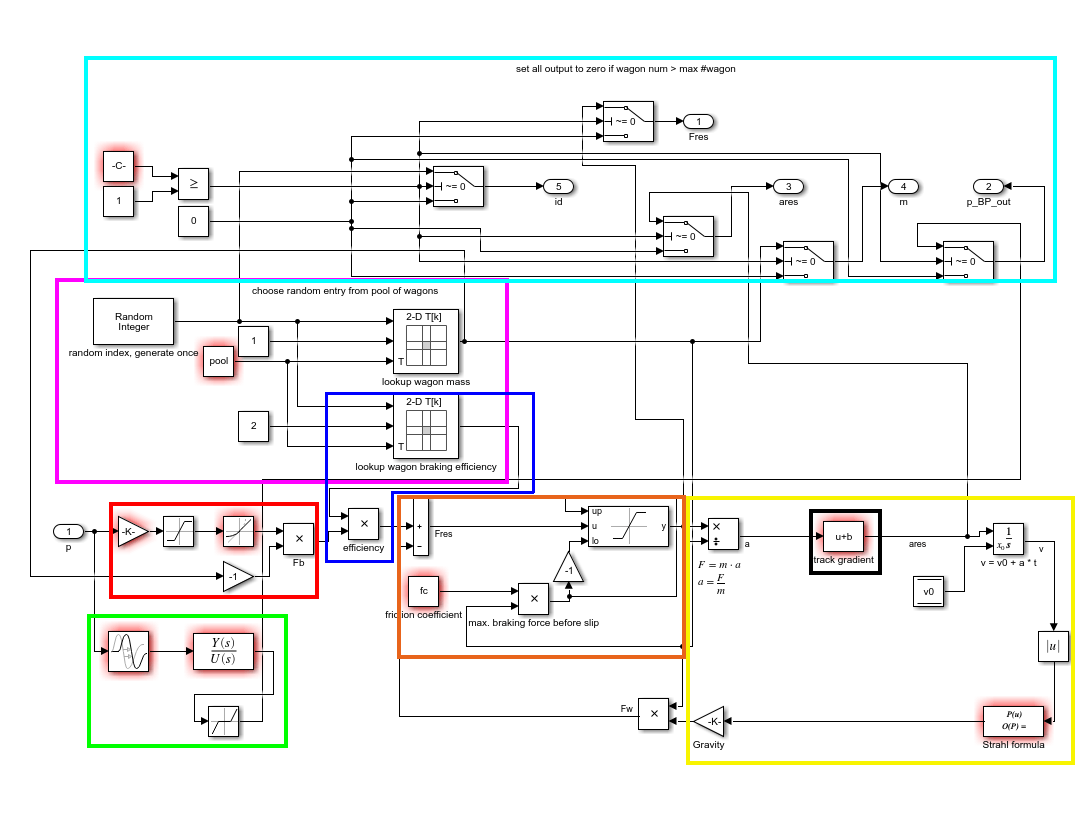
\includegraphics[width=\linewidth]{./pic/expandedmodel_wagon}
	\caption{Expanded Model - Wagon}
	\label{fig:expandedmodel_wagon}
\end{figure}

\par\noindent
The last subsystem is the actual wagon. We will take a look at the largely unchanged elements first. The sole input is still the braking pressure on the brake pipe. Simulation of the propagation delay has also remained the same as before. 

\par
One new addition is a pool of different wagons. Whereas before all 40 were distinguishable only by their position, they are now assigned with different parameters. To that end, a pool of 500 wagons has been randomly generated via python script, where each wagon has a unique ID, as well as randomly generated mass and braking efficiency. In actual simulation, up to 40 of these 500 are, currently by generation of random indices, selected and their properties used accordingly. It would also be possible to determine the wagon ids to be used beforehand, instead of choosing randomly.

\par
Another requirement was to make the number of wagons variable. In the initial model, the modeled train had a fixed number of 40 wagons, therefore also 40 wagon subsystems. Unfortunately, simulink offers no way to disable certain subsystems dynamically, but only by manually turning them off via model explorer, which would be unfeasible for such a large number of simulations. To circumvent this issue, output gets disabled for all unwanted wagons. For a simulation of a train of 20 wagons, the first 20 remain untouched, while the latter 20 produce no output and therefore also have no impact on the overall simulation. The turning off is achieved by simple switches; each wagon subsystem has a unique index from one to forty. If the index is greater than the specified number of wagons, all switches are turned to output zero.
	
\section{Further Expansion}
\label{sec:FurtherExpansion}